\documentclass[11pt]{book}

%%Magyar nyelvi beállítások és extra csomagok
\usepackage[magyar]{babel}
\usepackage{t1enc}
\usepackage{hulipsum}
\usepackage{graphicx}
\usepackage{wrapfig}
\usepackage{subcaption}
\usepackage{xcolor}

%%Oldalbeállítások, header, footer
\usepackage{fancyhdr}
\pagestyle{fancy}
\fancyhead[OL]{\nouppercase\rightmark}
\fancyhead[OR]{}
\fancyhead[ER]{\nouppercase\leftmark}
\fancyhead[EL]{}
\fancyfoot[ER]{\thepage}
\fancyfoot[OL]{\thepage}
\fancyfoot[C]{}
\setlength{\headheight}{13.59999pt}
\fancypagestyle{plain}{%
\fancyhf{}% %minden mező törlése
\fancyfoot[ER]{\thepage}
\fancyfoot[OL]{\thepage}
\fancyfoot[C]{}}

%%Matematika
\usepackage{amsmath} 
\usepackage{mathtools} 
\usepackage{amsfonts} 
\usepackage{amsthm} 
\theoremstyle{definition} 
\newtheorem{tet}{Tétel}
\newtheorem{defin}{Definíció}
\usepackage{chngcntr}
\counterwithout{equation}{chapter}

%%Programozás
\usepackage{algpseudocode} 
\usepackage{algorithm} 
\floatname{algorithm}{Algoritmus}
\usepackage{listings}
\usepackage{float}
\usepackage{newfloat}

%%Egyéni környezet
\newenvironment{modverse}[2]%
{%
	\begin{verse}
	\begin{center}
	\textbf{#1} \\
	\textit{#2} \\[0.5cm]
	
}%
{\end{center}\end{verse}}

\begin{document}

\title{Zárthelyi dolgozat \\A csoport} 
\author{Nagy Balázs EIO1RQ}
\date{\today}
\maketitle



\chapter{Oldalbeállítások}

\section{Első szekció}
\hulipsum[1-10]

\section{Második szekció}
\hulipsum[1-10]

\chapter{Képek}

\hulipsum[1-6]

\begin{wrapfigure}{r}{0.5\textwidth}
\caption{\textbf{Képek}}
	\begin{flushright}
		
\includegraphics[height=4cm, keepaspectratio]{szines}
		\caption{Színes}
	\end{flushright}
	\begin{flushright}
		\fcolorbox{black}{blue}{\scalebox{-1}								{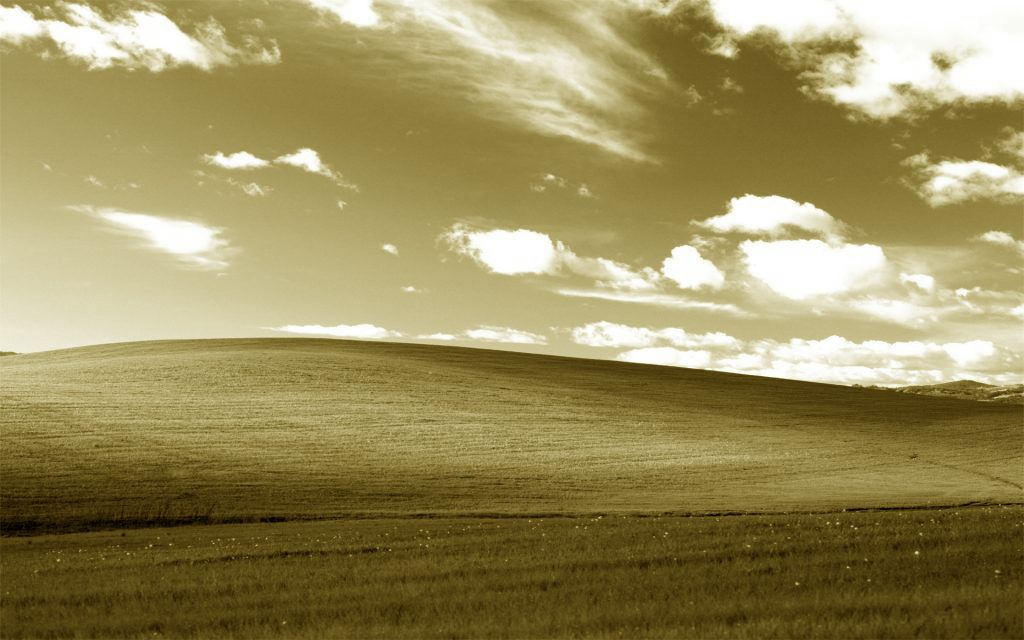
\includegraphics[height=4cm, keepaspectratio]{szepia}}}
		\caption{Szépia}
	\end{flushright}
\end{wrapfigure}

\hulipsum[1-6]

\chapter{Matematika}

\begin{defin}[Sajátérték]
Legyen $A \in \mathbb{R}^{n \times n}$ négyzetes mártix. Azt mondjuk, hogy $\lambda \in \mathbb{C}$ sajátértéke és $v \in \mathbb{C}^n$ a $\lambda$ sajátértékhez tartozó (jobb oldali) sajátvektora $A$-nak, ha

\begin{equation}
Av = \lambda v
\end{equation}
\end{defin}

\begin{defin}[Karakterisztikus polinom]
Jelülje $E \in \mathbb{R}^{n \times n}$ az egységmátrixot.
Az $A$ ún. \textit{karakterisztikus polinomja}

\begin{equation}
\varphi(\lambda):=det(A\textcolor{red}{-\lambda E})= \begin{vmatrix}
a_{11} \textcolor{red}{-\lambda} & a_{12} & \cdots & a_{1n} \\
a_{21} & a_{22} \textcolor{red}{-\lambda} & \cdots & a_{2n} \\
\vdots & \vdots & \ddots & \vdots \\
a_{n1} & a_{n2} & \cdots & a_{nn} \textcolor{red}{-\lambda} \\
\end{vmatrix},
\end{equation}
egy $n$-ed fokú polinom $\lambda$-ban.
\end{defin}

\begin{tet}{Sajátérték meghatározása}
Az $A \in \mathbb{R}^{n \times n}$ mátrix sajátértékei az ún. \textit{karakterisztikus egyenlet}
\begin{equation}
\varphi(\lambda) = 0
\end{equation}
megoldásai. Mivel a $\varphi(\lambda)$ \textit{karakterisztikus polinom} egy $n-$edfokú polinom $\lambda$-ban,
ezért a komplex számokon (multiplicitással együtt) $n$ megoldása van.
\end{tet}

\chapter{C kód}

\hulipsum[1-8]

\begin{center}
\lstset{%
    caption=Descriptive Caption Text,
    basicstyle=\ttfamily\footnotesize\bfseries,
    frame=tb
  }
\begin{minipage}{\textwidth}
\begin{lstlisting}[language=c, numbers=right, showspaces=true, stepnumber=2, tabsize=2, frame=tlBR, caption={Bináris keresés C-ben}]
binarySearch(arr, x, low, high){
	repeat till low = high
		mid = (low + high)/2
			if (x == arr[mid])
				return mid;

			else if (x > arr[mid])	// x is on the right side
				low = mid + 1;

			else			// x is on the left side
				high = mid - 1;
}
\end{lstlisting}
\end{minipage}
\end{center}

\hulipsum[1-8]

\chapter{Vers környezet}

\begin{modverse}{Kép a tükörben}{József Attila}
Hogyan volt, azt már nem tudom.\\
De mégis csak megláttam egyszer,\\
Bámultam rája nagy szemekkel.\\
Már régen volt, csak ezt tudom.\\[0.5cm]

Néztem égve.\\
Arca, alakja tűztükörbe,\\
Szemembe rögződött örökre\\
S szivemre hajlott tündökölve.\\
\end{modverse}


\chapter{Ciklus -- bónusz feladat}

\newcounter{index}
\setcounter{index}{1}
\whiledo{\value{index}<61}
{%
\ifodd \theindex {\textcolor{black}{\theindex}} \else {\textcolor{red}{\theindex}} \fi
\stepcounter{index}%
}

\end{document}